\chapter{なくしもの発生確率の導出}

% 付録です. 
$ p_{t i} = \mathrm{P}(\tau = t , m_t = M_i) $とおけば
\begin{equation} \label{eq:p_sum_pt}
    p_i = \sum_{t=1}^{\infty}p_{t i}
\end{equation}
である.

$ p_{t i} $を求めるにあたって,まず$ q_{t i} = \mathrm{P}(\tau > t\ ,m_t = M_i) $の一般項を求める.
$ q_{t i} $は次の漸化式を満たす.
\begin{align*}
    q_{t+1 i} & = \! \sum_{k} \mathrm{P}(\tau \! > \! t + 1\ , m_{t+1} \! = \! M_i\ , m_t \! = \! M_k) \\
    & = \! \sum_{k} \mathrm{P}(\tau \! \ne \! t + 1 , m_{t+1} \! = \! M_i , m_t \! = \! M_k | \tau \! > \! t) \mathrm{P}(\tau \! > \! t) \\
    & = \! \sum_{k} \left(
        \begin{array}{l}
            \mathrm{P}(\tau \! \ne \! t + 1 | \tau \! > \! t , m_{t+1} \! = \! M_i , m_t \! = \! M_k) \\
            \times \mathrm{P}(m_{t+1} \! = \! M_i , m_t \! = \! M_k | \tau \! > \! t) \mathrm{P}(\tau \! > \! t)
        \end{array}
    \right) \\
    & = \! \sum_{k} \left(
        \begin{array}{l}
            \mathrm{P}(\tau \! \ne \! t + 1 | \tau \! > \! t , m_{t+1} \! = \! M_i , m_t \! = \! M_k) \\
            \times \mathrm{P}(m_{t+1} \! = \! M_i , m_t \! = \! M_k) \mathrm{P}(\tau \! > \! t)
        \end{array}
    \right) \\
    & = \! \sum_{k} \left(
        \begin{array}{l}
            \mathrm{P}(\tau \! \ne \! t + 1 | \tau \! > \! t , m_{t+1} \! = \! M_i , m_t \! = \! M_k) \\
            \times \mathrm{P}(m_{t+1} \! = \! M_i | m_t \! = \! M_k) \mathrm{P}(m_t \! = \! M_k) \mathrm{P}(\tau \! > \! t)
        \end{array}
    \right) \\
    & = \! \sum_{k} \left(
        \begin{array}{l}
            \mathrm{P}(\tau \! \ne \! t + 1 | \tau \! > \! t , m_{t+1} \! = \! M_i , m_t \! = \! M_k) \\
            \times \mathrm{P}(m_{t+1} \! = \! M_i | m_t \! = \! M_k) \mathrm{P}(\tau \! > \! t , m_t \! = \! M_k)
        \end{array}
    \right) \\
    & = \! \sum_{k \ne i} (1 - \theta_i) a_{k i} q_{t k} + a_{i i} q_{t i}
\end{align*}
$ q_t = (q_{t 1} , q_{t 2} , \cdots , q_{t n})^\mathrm{T} $とおいて行列で書けば
\begin{equation*}
    \arraycolsep3pt
    q_{t + 1} \! = \!
    \begin{pmatrix}
        a_{1 1} & (1 \! - \! \theta_1) a_{2 1} & \cdots & (1 \! - \! \theta_1) a_{n 1} \\
        (1 \! - \! \theta_2) a_{1 2} & a_{2 2} & \cdots & (1 \! - \! \theta_2) a_{n 2} \\
        \vdots & \vdots & \ddots & \vdots \\
        (1 \! - \! \theta_n) a_{1 n} & (1 \! - \! \theta_n) a_{2 n} & \cdots & a_{n n} \\
    \end{pmatrix}
    \! q_t
\end{equation*}
となる.この係数行列を$ K $とおけば
\begin{equation} \label{eq:recur}
    q_{t + 1} = K q_t
\end{equation}
である.また初項$ q_{1 i} $についても$ \mathrm{P}(\tau > 0) = 1 $であることに注意すれば同様にして下式を得る.
\begin{align*}
    q_{1 i} & = \! \sum_{k} \left(
        \begin{array}{l}
            \mathrm{P}(\tau \ne 1 | \tau > 0 , m_1 = M_i , m_0 = M_k) \\
            \times \mathrm{P}(m_1 = M_i | m_0 = M_k) \mathrm{P}(m_0 = M_k)
        \end{array}
    \right) \\
    & = \! \sum_{k \ne i} (1 - \theta_i) a_{k i} s_k + a_{i i} s_i
\end{align*}
これを$ s = (s_1 , s_2 , \cdots , s_n)^\mathrm{T} $とおいて行列で書けば
\begin{equation} \label{eq:init}
    q_1 = K s
\end{equation}
である.よって(\ref{eq:recur}),(\ref{eq:init})から$ q_t $の一般項は
\begin{equation} \label{eq:qt}
    q_t = K^t s
\end{equation}
となる.

次に$ p_{t i} $の一般項について,$ q_{t i} $の漸化式を求めたのと同様にして下式を得る.
\begin{align*}
    p_{t+1 i} & = \! \sum_{k} \mathrm{P}(\tau = t + 1 , m_{t+1} = M_i , m_t = M_k) \\
    & = \! \sum_{k} \left(
        \begin{array}{l}
            \mathrm{P}(\tau \! = \! t + 1 | \tau \! > \! t , m_{t+1} \! = \! M_i , m_t \! = \! M_k) \\
            \times \mathrm{P}(m_{t+1} \! = \! M_i | m_t \! = \! M_k) \mathrm{P}(\tau \! > \! t , m_t \! = \! M_k)
        \end{array}
    \right) \\
    & = \! \sum_{k \ne i} \theta_i a_{k i} q_{t k}
\end{align*}
これを$ p_t = (p_{t 1} , p_{t 2} , \cdots , p_{t n})^\mathrm{T} $とおいて行列で書けば
\begin{equation*}
    \arraycolsep3pt
    p_{t + 1} = 
    \begin{pmatrix}
        0 & \theta_1 a_{2 1} & \cdots & \theta_1 a_{n 1} \\
        \theta_2 a_{1 2} & 0 & \cdots & \theta_2 a_{n 2} \\
        \vdots & \vdots & \ddots & \vdots \\
        \theta_n a_{1 n} & \theta_n a_{2 n} & \cdots & 0 \\
    \end{pmatrix}
    q_t
\end{equation*}
となる.この係数行列を$ L $とおき(\ref{eq:qt})を代入すれば
\begin{equation} \label{eq:pt}
    p_t = L K^{t - 1} s
\end{equation}
である.

\begin{figure}[bt]
    \centering
    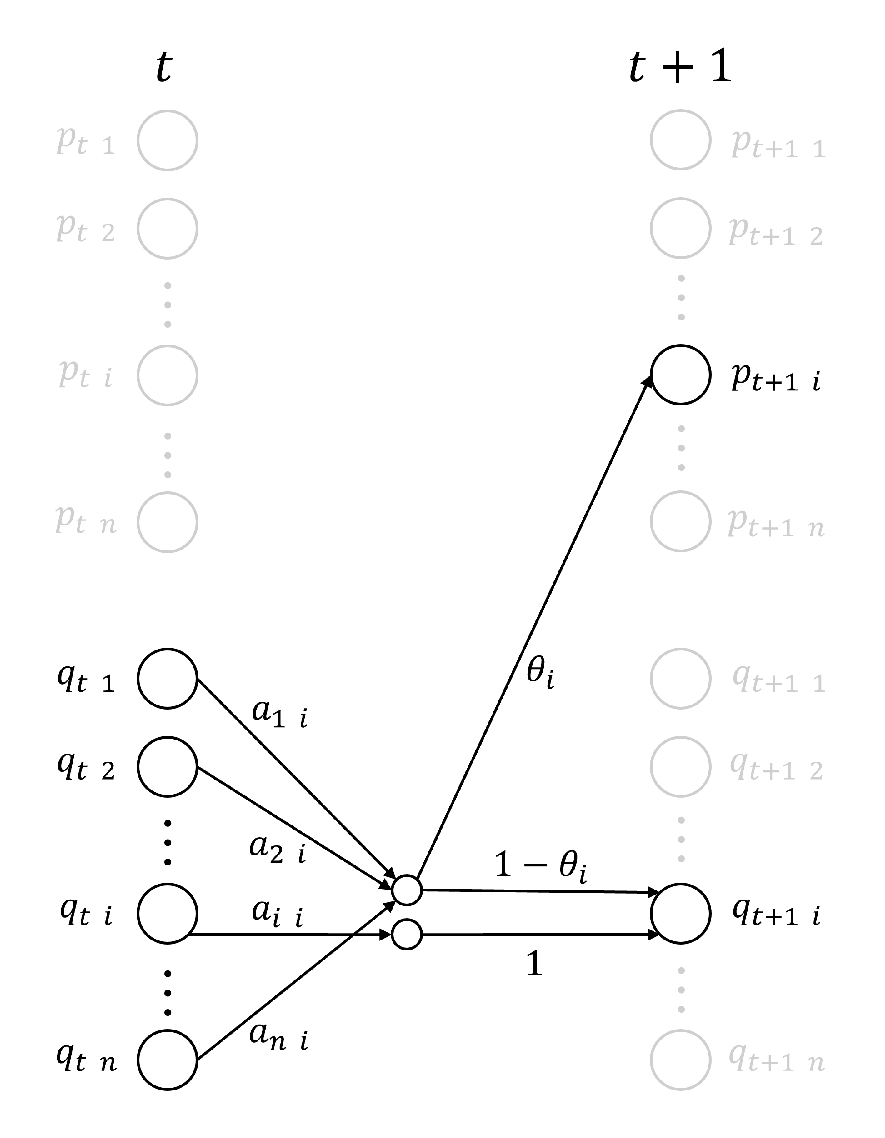
\includegraphics[keepaspectratio, width=0.7\linewidth]{figs/pq.eps}
    \caption{A diagram representing the recurrence formula of $ p_{t i} $ and $ q_{t i} $}
\end{figure}

次に$ p_i $について,$ p = (p_1 , p_2 , \cdots , p_n)^\mathrm{T} $とおき(\ref{eq:pt})を(\ref{eq:p_sum_pt})に代入すれば
\begin{align}
    p &= \sum_{t=1}^{\infty} L K^{t - 1} s \nonumber \\
    &= L \left( \sum_{t=0}^{\infty} K^t \right) s \label{eq:p_}
\end{align}
を得る.

ここで$ \sum K^t $が収束することを示す.
ゲルシュゴリンの定理\cite{s_saito}より$ K^\mathrm{T} $の任意の固有値$ \lambda $はいずれかの$ i $に対し
\begin{equation*}
    a_{i i} - \sum_{j \ne i}(1 - \theta_j) a_{i j} \le \lambda \le a_{i i} + \sum_{j \ne i}(1 - \theta_j) a_{i j}
\end{equation*}
を満たす.右の不等式についてマルコフ連鎖がエルゴード的であることから$ a_{i i} < 1 $\cite{funaki}であり,$ \theta_j > 0 $でもあるので
\begin{equation*}
    \lambda < a_{i j} + \sum_{j \ne i} a_{i j} = 1
\end{equation*}
となる.同様に左の不等式についても
\begin{equation*}
    \lambda > -1
\end{equation*}
となる.よって$ K^\mathrm{T} $の固有値はいずれも絶対値が$ 1 $未満である.すると$ K $と$ K^\mathrm{T} $の固有値は等しいので$ K $の固有値も絶対値が$ 1 $未満となる.
よって行列等比級数の公式\cite{m_saito}が使えて
\begin{equation} \label{eq:sumK}
    \sum_{t=0}^{\infty} K^t = (I - K)^{-1}
\end{equation}
となる.ただし$ I $は$ n $行$ n $列の単位行列である.

(\ref{eq:sumK})を(\ref{eq:p_})に代入すれば(\ref{eq:p})を得る.

$ p_i $を重みとした$ h_i $の和
\begin{equation} \label{eq:h}
    h = p_1 h_1 + p_2 h_2 + \cdots + p_n h_n
\end{equation}
をなくしものの位置分布とする.

\subsection{遷移確率と位置分布の学習}
マルコフ連鎖とヒートマップの組み合わせが連続型HMM(Hidden Markov Model)に類似していることに注目する.
HMMのパラメータ学習アルゴリズムにBaum-Welchアルゴリズムがある.\cite{ishii_ueda}
$ h_i $が多変量ガウス分布であるという制約の下,利用者の位置を監視しBaum-Welchアルゴリズムを適用することで$ a_{i j} $と$ h_i $を同時に学習する.

\subsection{遷移失敗確率の学習} \label{ss:faultprob}
ベイズ推論を用いる.
なくしものの発見場所を$ x_{\mathrm{found}} $,$ \theta = (\theta_1 , \theta_2 , \cdots , \theta_n)^\mathrm{T} $の事前分布の密度関数を$ f $とおく.
$ \theta $の分布の更新にあたり尤度としてなくしものの位置分布$ h $を用いる.すなわち更新事後分布の密度関数$ f(\theta | x_{\mathrm{found}}) $を下式で定める.
\begin{equation} \label{eq:new_f}
    f(\theta | x_{\mathrm{found}}) \propto h(x_{\mathrm{found}} , \theta) f(\theta)
\end{equation}
ただし$ h $を$ x \in X $と$ \theta $の関数とみなしている.

\subsection{推定}
\begin{equation} \label{eq:exp}
    \mathrm{E}_\theta [h] = \int_{0}^{1} \int_{0}^{1} \cdots \int_{0}^{1} h f(\theta) \mathrm{d}\theta_1 \mathrm{d}\theta_2 \cdots \mathrm{d}\theta_n
\end{equation}
を推定結果とする.
